\documentclass[12pt]{article}
%\usepackage{times}
\usepackage{graphicx}
\usepackage{gensymb}
\usepackage{amsmath}
%\usepackage{trackchanges} %Paket für Änderungen nachverfolgen:
    %\note[Person]{Kommentar}
    %\annote[Person]{Textstelle}{Kommentar}
    %\add[Person]{ergänzte Textstelle}
    %\remove[Person]{gelöschte Textstelle}
    %\change[Person]{gelöschte Textstelle}{ergänzte Textstelle}
\usepackage{booktabs}
\usepackage{colortbl}
\usepackage{xcolor}
\usepackage{xfrac}
  
\usepackage[right]{lineno} %Line Numbers
\usepackage[breaklinks=true,urlcolor=blue,colorlinks=true,citecolor=black,linkcolor=blue]{hyperref}
\usepackage[english]{babel}

\usepackage[style=nature, backend=bibtex]{biblatex}
\addbibresource{library.bib}

\urlstyle{same}
\topmargin 0.0cm
\oddsidemargin 0.2cm
\textwidth 16cm 
\textheight 21cm
\footskip 2.0cm
\setlength{\parindent}{1cm}

\makeatletter\renewcommand{\@biblabel}[1]{#1.}\makeatother

\date{}


\begin{document}
\renewcommand{\baselinestretch}{2}

%title
\begin{center}\normalsize\textsc{Predictive Coding and Bistable Perception}\\
\LARGE The Role of Inferior Frontal Cortex in Bistable Perception\\\vspace*{24pt}


%authors
\large Veith Weilnhammer$^{1,\ast}$, Katrin Reichenbach$^{1}$, Philipp Sterzer$^{1, 2, 3} $\vspace*{24pt}\\
%affiliations
\footnotesize$^{1}$Department of Psychiatry, Charit\'{e} Universit\"{a}tsmedizin Berlin, 10117 Berlin, Germany\\

$^{2}$Bernstein Center for Computational Neuroscience, Charit\'{e} Universit\"{a}tsmedizin Berlin, 10117 Berlin, Germany\\
$^{3}$Berlin School of Mind and Brain, Humboldt-Universit\"{a}t zu Berlin, 10099 Berlin, Germany\\ \vfill

%corresponding
{\begin{minipage}[b]{\textwidth} $^\ast$	
Corresponding author:  Veith Weilnhammer, Department for Psychiatry and Psychotherapie, Charit\'{e} Campus Mitte, Charit\'{e}platz 1, 10117 Berlin, phone: 0049 (0)30 450 517 317, email: veith-andreas.weilnhammer@charite.de\\ 
\end{minipage}}
\end{center}


\linenumbers

%%%%%%%%%%%%%%%%%%%%%%%%%%%%%%%%%%%%%%%%%%%%%%%%%%%%%%%%%%%%%%%%
%ABSTRACT
\renewcommand{\baselinestretch}{1.5}\normalsize

\clearpage
\section*{Abstract}

One of the most debated topics in cognitive neuroscience concerns the role of frontal cortex in conscious perception. Research on bistable perception, the spontaneous alternation between two perceptual states that occurs when sensory information is ambiguous, has repeatedly fuelled this debate. In particular, an on-going controversy revolves around the question whether the inferior frontal cortex (IFC) is causally involved in perceptual transitions during bistable perception.  Here, we draw on the framework of predictive coding to propose that IFC activity reflects the mismatch (i.e., prediction error) between perceptual content and sensory evidence, thereby driving perceptual alternations.  To test this hypothesis, we introduce the novel paradigm of graded ambiguity, which relies on a manipulation of sensory evidence for the two perceptual interpretations of a bistable structure-from-motion stimulus. Using pilot data, behavioral modeling and data simulations, we develop quantitative predictions for the modulation of prediction errors and associated brain activity by graded manipulations of sensory evidence. After preregistration, we will use functional magnetic resonance imaging to test the prediction that IFC activity scales with prediction errors evoked by the mismatch between perception and sensory evidence. The expected results will help to settle a long-standing debate regarding the role of frontal cortex in bistable perception and, more generally, in conscious perceptual experience. Our study therefore has the potential to fundamentally advance our understanding of the neural underpinnings of consciousness.

%%%%%%%%%%%%%%%%%%%%%%%%%%%%%%%%%%%%%%%%%%%%%%%%%%%%%%%%%%%%%%%%
%MAIN TEXT
\renewcommand{\baselinestretch}{1.5}\normalsize

\clearpage
\section{Introduction}

The role of frontal brain areas in conscious perceptual experience is currently one of the most disputed topics in the neuroscientific study of consciousness. Most prominently, an ongoing debate has revolved around the question whether neural activity in frontal brain areas is causally involved in enabling conscious perception \parencite{Odegaard2017, Boly2017}.

A key experimental approach that has been in the focus of the controversy regarding the neural mechanisms of conscious visual experience is based on the phenomenon of bistable perception \parencite{Brascamp2018}. Such bistable perception occurs when observers view an ambiguous stimulus that is compatible with two mutually exclusive perceptual interpretations, typically resulting in fluctuations between the two possible percepts. Transitions between the two perceptual states occur spontaneously and in the absence of any change in visual stimulation. Importantly, these transitions thus mark a process by which our perceptual system establishes an unambiguous perceptual experience in the light of ambiguous sensory information \parencite{Sterzer2009, Hohwy2008a}. Thereby, bistable perception highlights a fundamental aspect of perception: As our brains do not have direct access to the events in the world, they constantly face the task of inferring the states of the world form the inherently ambiguous data registered by our sensory organs. This process of perceptual inference has been proposed to engender conscious perception in general \parencite{Hohwy2012} and transitions during perceptual bistability in particular \parencite{Sterzer2007, Hohwy2008a}. Transitions in bistable perception hence provide a unique window onto the nature of conscious experience and its relation to neural activity in frontal brain areas \parencite{Odegaard2017, Boly2017}.

Over the past two decades, the controversy regarding the implication of frontal brain activity in conscious experience has therefore reverberated in research on the neural processes involved in perceptual transitions during bistability. Several functional neuroimaging studies in humans have pointed to a key role of a region in the right inferior frontal cortex (IFC), which consistently showed greater neural activity in association with perceptual transitions during bistability as compared to perceptual events evoked by changes in visual stimulation \parencite{Brascamp2018}. However, the precise role of the IFC in bistable perception is still a matter of debate, as it has remained elusive whether activity in this area constitutes a potential cause (\textit{top-down}, \cite{Sterzer2007, Lumer1998, Weilnhammer2013}) or rather the consequence (\textit{bottom-up}, \cite{Knapen2011, Frassle2014, Brascamp2015}, see Figure 1A) of spontaneous changes in the contents of conscious perception.

Our current work aims to resolve the apparent conflict between these two views and to thereby elucidate the relationship between frontal brain activity and conscious perception. To this end, we draw on previous theoretical and empirical work suggesting that the opposing views of IFC activity as reflecting either a top-down or a bottom-up mechanism may be reconciled within the framework of predictive coding, which models perception as Bayesian inference within a hierarchical predictive system \parencite{Hohwy2008a, Weilnhammer2017, Brascamp2018}. According to this influential theory, our brain entertains a generative model of the sensory environment. Predictions derived from this model are sent from higher to lower levels of the processing hierarchy via feedback (i.e., \textit{top-down}), thereby enabling inferences regarding the causes of sensory data \parencite{knill_bayesian_2004, Friston2005, Clark2013}. If the internal model fails to predict incoming sensory data, the resulting prediction errors (PE) propagate to higher hierarchical levels in a feed-forward manner (i.e., \textit{bottom-up}) and update the model. The constant updating of the internal generative model through inference thereby serves the purpose of PE minimisation \parencite{Hohwy2012}. 

How can this notion of PE minimisation account for the occurrence of perceptual transitions during bistable perception \parencite{Sundareswara2008, Gershman2012}? According to a predictive-coding model of bistable perception \parencite{Hohwy2008a, Weilnhammer2017}, conscious perception represents the best hypothesis regarding the cause of currently available sensory information, that is, the hypothesis that is best at minimising PE. However, if the available sensory information is ambiguous and hence equally compatible with two (mutually exclusive) hypotheses, a prediction based on one of these hypotheses will never fully account for sensory information. According to the predictive conding model, residual evidence for the alternative perceptual hypothesis thus constitutes a PE, which accumulates over time and thereby destabilises the current percept. This eventually results in a transition to the other possible percept (see Figure 1B, \cite{Weilnhammer2017}). Crucially, predictive coding theorizations therefore understand perceptual transitions as an attempt to minimise PE by re-attributing the sensory input to the alternative perceptual hypothesis. 

Here, we suggest that this predictive coding model can help us to understand the functional significance of frontal activity during bistable perception. Specifically, we propose that the previously reported transition-related activity in the IFC \parencite{Brascamp2018} may reflect the accumulation of PE in a process that culminates in a perceptual transition. This notion may reconcile the above-mentioned bottom-up and top-down views on transition-related IFC activity: On the one hand, activity in the IFC may reflect the build-up of PEs that originate from early processing stages and propagate up the hierarchy to frontal cortex in a bottom-up manner. On the other hand, the IFC may in turn engender a top-down modulation of activity in visual cortex that facilitates a perceptual transition, thereby minimising PE \parencite{Weilnhammer2013, Brascamp2018}. In a recent proof-of-concept study using model-based functional magnetic resonance imaging (fMRI), we confirmed that PE time-courses derived from a Bayesian predictive-coding model of bistable perception indeed correlated with neural activity in the IFC \parencite{Weilnhammer2017}. Importantly, activity in IFC showed a gradual increase towards perceptual transitions, in line with the notion that PE accumulates over time before it is minimised by virtue of a perceptual transition. As the PE therefore peaks at each perceptual transition (see Figure 1B), it is tempting to speculate that the oft-reported finding of transition-related IFC activity \parencite{Brascamp2018} actually reflects these peaks.  

In the present study, we will directly test the hypothesis that activity within the IFC represents a PE signal that stems from neural activity coding for the currently suppressed interpretation of the ambiguous input and thereby plays a pivotal role in the resolution of ambiguity in conscious perception. Our rationale is to experimentally manipulate the available sensory evidence that favours one of the two alternative perceptual hypotheses. This modulates the strength of PEs during periods in which the corresponding percept is suppressed. In the presence of such additional sensory evidence in form a graded disambiguating signal, the PE dynamics should change as follows: If the observer adopts a percept that is congruent with the disambiguating sensory evidence, PEs will be reduced and perceptual transitions to the alternative percept less likely. Conversely, if the observer adopts a percept that is incongruent with the disambiguating sensory evidence, PEs will be enhanced and perceptual transitions to the alternative percept become more likely (see Figure 1B). The effectiveness of this modulation depends on the amount of available disambiguating sensory evidence. 

To test these predictions, we developed a novel fMRI paradigm based on bistable perception with graded perceptual ambiguity, which parametrically disambiguates structure-from-motion stimuli by introducing varying degrees of sensory evidence for one over the other percept. We first present data from a pilot experiment as proof-of-concept for this experimental manipulation of graded perceptual ambiguity. Furthermore, we simulate data from a predictive-coding model of bistable perception in order to illustrate the expected modulation of neural activity by varying degrees of sensory evidence during perceptual bistability, which we will assess in an fMRI-experiment that will be conducted in an independent group of participants after pre-registration.

We hypothesize that PE related fMRI signals in IFC reflect the incongruency between the currently dominant perceptual interpretation and the available sensory evidence. In other words, we expect lower IFC activity during congruency between the sensory evidence and the current percept (reduced PEs) and higher activity during incongruency between the two (enhanced PEs). Crucially, we predict that varying degrees of sensory evidence modulate the assumed effect of congruency: Differences in neural activity between incongruent and congruent perceptual phases should scale with the available amount of disambiguating sensory evidence. Of note, we thus assess the role of IFC in perceptual bistability by probing its activation as a function of congruency of perception with sensory evidence, rather than in direct relation to perceptual transitions.

In sum, we strive to expand our knowledge about the frequently debated functional significance of frontal brain activity during bistable perception by probing the interaction between perceptual congruency and sensory evidence in the IFC. Critically, our experimental design will enable us to elucidate the controversial role of IFC in perceptual transitions by directly testing the supposed underlying mechanism based on PE signalling. This allows us to circumvent any confounding effects of perceptual reports that have afflicted many previous studies directly measuring the neural correlates of perceptual transitions \parencite{Tsuchiya2016}. We believe that this study will help to settle a long-standing debate regarding the role of frontal brain areas in bistable perception and, more generally, in the inferential processes that give rise to conscious perception.

\section{Results}

\subsection{Pilot Data}

We report data from a pilot experiment in $n = 10$ participants to provide a proof-of-concept for our novel experimental paradigm of perceptual bistability during graded ambiguity. Furthermore, we use simulations from the predictive coding model of bistable perception to exemplify the expected effects of our experimental manipulation on PEs during perceptual bistability.

\subsubsection{Conventional Analyses}

Firstly, we verified that varying levels of sensory evidence introduced by graded ambiguity impact on the sequence of perceptual states during bistability. This effect is captured by the dependent variable "congruent percepts" (i.e., the fraction of percepts congruent with current sensory evidence), which we expected to vary according to the level of disambiguating sensory evidence. Secondly, we asked whether the graded ambiguity manipulation has an influence on temporal and qualitative aspects of bistable perception. These are reflected by the dependent variables "average phase durations" (i.e., the average time spent between transitions in perception) and "fraction of unclear percepts" (i.e., the proportion of percepts reported as "unclear" as opposed to clear perceptual interpretations of the stimulus), respectively. 
Average perceptual phase durations amounted to 15.79 $\pm$ 0.50 sec. Participants reported a fraction of 0.03 $\pm$ 0.01 of percepts as perceptually "unclear". For both dependent variables, we did not observe a main effect of sensory evidence as indicated by one-way repeated-measures analysis of variance (rmANOVA; average perceptual phase: $F(9) = 0.28$, $p = 0.96$; unclear percepts: $F(9) = 1.45$, $p = 0.20$). For the dependent variable "congruent percepts", one-way rmANOVA showed the expected main effect of sensory evidence ($F(9) = 17.50$, $p < 1.3e-10$, see Figure 2A).

\subsubsection{Model-based Analyses}
We furthermore transferred the results from the conventional analyses onto the predictive coding model of bistable perception (see Methods and Figure 4 for a detailed description). In this model, the initial precision of a prior distribution "perceptual stability" ($\pi_{IPS}$) captures the individual average phase duration. The precision of the likelihood distribution "disambiguation" ($\pi_{DIS}$), in turn, mirrors the impact of sensory evidence on perceptual states during graded ambiguity. We first established the relevance of both likelihood and prior precision for the sequence of perceptual states during bistability using Bayesian Model Comparison (BMC). We then assessed a potential effect of our experimental manipulation on the individual participants’ estimates for prior and likelihood precision using frequentist statistics. 

In model-based analyses, random-effects BMC identified the winning-model (53$\%$ exceedance probability) to incorporate both the prior distribution "perceptual stability" and the likelihood distribution "disambiguation". The initial precision (all precision parameters in log space) of the perceptual stability prior $\pi_{IPS}$ amounted to 1.1244 $\pm$ 0.1449 with no effect of sensory evidence as indicated by one-way rmANOVA ($F(9) = 0.67818$, $p < 0.6679$). For the precision of "disambiguation", in turn, rmANOVA showed the expected main effect of sensory evidence ($F(9) = 9.3664$, $p < 8.4405e-07$, see Figure 2B).

Correlations between conventional and model-based analyses served as a sanity-check for model inversion. As expected, average phase durations correlated with average posterior $\pi_{IPS}$ ($\rho(9) = 0.85$, $p = 0.0018$, Pearson correlation, Figure 2C). Participant-wise correlation coefficients between congruent percepts and posterior $\pi_{DIS}$ (both variables computed separately for all levels parametric disambiguation) amounted to 0.86 $\pm$ 0.03 (one-sample one-sided t-test against zero: $T(9) = 29.4$, $p = 1.9537e-09$, inset Figure 2C).

\subsection{Simulation}
Finally, we provide simulations from our predictive coding model to illustrate the expected effect of graded ambiguity on perception and average PE estimates during perceptual bistability. As expected, we found a significant effect of sensory evidence on the fraction of congruent percepts ($F(46) = 37.635$, $p = 5.5585e-37$) as indicated by one-way rmANOVA (Figure 2D). With regard to average PEs (see Figure 2E), two-way rmANOVA with the factors "congruency" and "sensory evidence" showed a significant main effect of congruency ($F(46) = 186.540$, $p < 0.0001$) and a significant "congruency" by "sensory evidence" interaction ($F(46) = 55.380$, $p < 0.0001$). In addition, two-way rmANOVA indicated a significant main effect of "sensory evidence" on PEs ($F(46) = 41.705$, $p < 0.0001$).

\section{Methods}

Please note that all custom code (PsychToolbox and Matlab 2014b) relating to power analysis, presentation and analysis of the experiment as well as all behavioural and simulated pilot data are accessible on GitHub (\url{https://github.com/veithweilnhammer/Prereg_IFC_Bistability}).

\subsection{Participants}

\subsubsection{Pilot Experiment}

We recruited 12 participants (7 female, age: 19-32, corrected-to-normal vision, no prior neurological or psychiatric medical history). We excluded one participant due to an insufficient number of perceptual transitions and another participant due to below-threshold performance (see Exclusion criteria).

\subsubsection{fMRI Experiment: Power Analysis}

We determine the sample-size necessary to detect a modulated PE signal during perceptual bistability within IFC (Neuromorphometrics mask for right-hemispherical anterior insula and opercular/triangular inferior frontal gyrus, see \cite{Brascamp2018}, as provided by SPM12, \url{http://www.fil.ion.ucl.ac.uk/spm/software/spm12}) based on the second-level contrast "PE vs. baseline" from an independent dataset \parencite{Weilnhammer2017}. We restricted power-analyses to voxels that showed transition-related activity (second-level contrast "Transition vs. baseline" at a lenient threshold of 0.05, uncorrected) within anatomical IFC in that dataset. 

A-priori power-analysis (1-$\beta$ = 0.95, $\alpha$ = 0.05) using FMRIpower \parencite{Mumford2008} indicates a sample-size of 47 participants (after application of exlclusion criteria, female and male, right-handed, age 18 to 65, corrected-to-normal vision and no prior neurological or psychiatric medical history). 

\subsection{Experimental Procedures}

\subsubsection{Main Experiment}

In this study, participants view an ambiguous random-dot kinematogram (RDK, Figure 3). Random dots distributed in intersecting rings induce the perception of a spherical object rotating left- or rightward around a vertical axis \parencite{Pastukhov2012a}.  We introduce a novel paradigm based on graded ambiguity, which enables a parametric modulation of sensory evidence for the two stimulus interpretations during perceptual bistability. Separating presentation between the two eyes using red-and-blue filter-glasses (left eye: red channel, right eye: blue channel) enables us to present both ambiguous as well as partially disambiguated versions of the stimulus. We achieve graded disambiguation of the RDK by parametrically varying the fraction of dots associated with a stereo-disparity signal. 

\paragraph{Pilot Experiment}

Our pilot experiment serves as proof-of-concept for our behavioural paradigm of perceptual bistability during graded ambiguity. Furthermore, we leverage the pilot data in behavioural modelling and simulations to deduce quantitative predictions for later fMRI-analyses. 

We presented three experimental runs consisting in 14 blocks of 58.11 sec visual stimulation. In each run, participants viewed seven pairs of blocks with ambiguous and partially disambiguated RDKs, respectively (diameter: $15.86\degree$ visual angle, rotational speed: 11.76 sec per rotation, rotations per block: 5, interval between overlapping configurations: 1.47 sec; individual dot size: $0.12\degree$), separated by five sec fixation, on a CRT-Monitor (85 Hz, viewing distance: 60 cm , screen size: 36.5 x 27.5 cm, resolution: 1280 x 960 pixels, pixels per degree visual angle: 30.2868). During ambiguous blocks (condition a), we stimulated the monocular channels with identical RDKs. This yielded ambiguous sensory stimulation and induced the phenomenon of perceptual transitions typical of bistable perception. Participants responded via button-presses indicating changes in perceived direction of rotation (arrow-keys of a standard keyboard; index/ring finger: rotation of the front-surface to the left/right; middle finger: unclear direction of rotation).

Importantly, the temporal sequence of changes in disambiguating sensory evidence introduced in each subsequent block was derived from the alternations in rotation direction as reported by the participant during the preceding ambiguous block. We introduced such sensory evidence by means of a stereo-disparity signal (i.e., graded ambiguity) between the two monocular channels. To this end, we shifted a fraction of the dots (§3.125\%, 6.25\%, 12.5\%, 25\%, 50\%, 75\% and 100\%§; conditions d1 to d7 in random order) composing the RDK by a rotational angle of $1.8\degree$ in opposing directions between the two eyes. The direction of shift yields additional sensory evidence that partially disambiguates the stimulus with regard to the enforced direction of rotation. 

\paragraph{fMRI Experiment}

In the pre-registered fMRI experiment (see Figure 3), we will present four runs containing six blocks of 120 sec with either ambiguous or parametrically disambiguated RDKs (diameter: $15.86\degree$, rotational speed: 12 sec per rotation, rotations per block: 10, interval between overlapping configurations: 1.5 sec; individual dot size: $0.12\degree$) separated by ten sec fixation on a LCD-Monitor (60 Hz, viewing distance: 158 cm, screen size: 39 x 52 cm, resolution: 3840 x 2160 pixels, pixels per degree visual angle: 72.7714) on a screen at head-end of the MRI-scanner bore. Participants will indicate changes in perceived direction of rotation (standard fMRI button-box; index/ring finger: rotation of the front-surface to the left/right; middle finger: unclear direction of rotation).

In contrast to the pilot experiment, the first run (R1) will comprise only ambiguous visual stimulation (condition A).  Based on the distribution of perceptual phase durations within this run, we will determine the time-points of changes in sensory evidence for the upcoming four runs (R2-R4), where we will introduce disambiguating sensory evidence (i.e., graded ambiguity) by a stereo-disparity signal. To this end, we will shift a fraction of the dots composing the RDK (§15\%, 30\%, 45\%, 60\%, 75\% and 100\%§, conditions D1 to D6 in random order) by a rotational angle of $1.8\degree$ in opposing directions between the two eyes.

\subsubsection{Control Experiment}
Based on the results from the pilot experiment and our simulation analysis, we expect that increasing levels of sensory evidence lead to a shortening of perceptual phases in which participants experience a direction of rotation incongruent with the current direction of disambiguation. We will therefore conduct a control fMRI-experiment (run R5) to test for potential effects of the shortening of one perceptual state at the expense of the other. To this end, we will present dots moving left or right along horizontal trajectories distributed randomly over a circular aperture of the same size as the RDKs presented in R1-R4 ($15.86\degree$; individual dot size: $0.12\degree$). We will present six blocks of 120 sec stimulation with changes in the direction of coherent leftward or rightward dot motion. Participants will be instructed to indicate changes in motion direction by button-presses. In each individual participant, we will determine the time spent in stimulus-congruent and incongruent perceptual states during runs R2 to R4 of the main experiment, separately for conditions D1 to D6. This temporal imbalance will inform the presentation time of one direction of coherent random dot motion relative to the other in six control conditions (C1 to C6). We will introduce changes in the direction of planar dot motion such that the experimental sequence will satisfy both the temporal imbalance between congruent and incongruent perceptual phases as well as the average individual transition frequency observed in the main experiment. We will randomize the direction of motion (left- vs. rightward motion) associated with reduced presentation time across conditions.  

\subsubsection{Behavioural Pre-Test}
Prior to the fMRI-experiment, participants will perform a short behavioural pre-test. Firstly, this experiment will serve to ascertain stereovision. Secondly, it will enable us to exclude participants who do not perceive an amount of perceptual transitions during bistability necessary for meaningful fMRI analyses (see Exclusion criteria below).  In these two consecutive pre-rest runs, we will present six blocks of 120 sec with either ambiguous or fully disambiguated RKDs (in analogy to runs R1 and R2-R4) separated by 5 sec fixation on a CRT- Monitor (see above), while participants report perceptual transitions.  

We will conduct a third pre-test run in participants who will participate in the fMRI-experiment. Here, we will assess potential differences in perceptual quality between congruent and incongruent perceptual states across the six levels of disambiguating sensory evidence. We will present six blocks of 120 sec with parametrically disambiguated RDKs (in analogy to runs R2-R4 from the main experiment), separated by 5 sec fixation. Participants will report perceptual transitions between congruent and incongruent perceptual states. Crucially, we will interrupt the stimulus presentation to collect ratings of perceptual quality on a four-point scale (1: "clear", 2: "rather clear", 3: "rather unclear", 4: "unclear") separately for congruent and incongruent percepts.

\subsubsection{Heterochromatic Flicker Photometry}
We will use red-blue-filter glasses to enable stereoscopic presentation. To avoid biases in the perceived direction rotation of structure-from-motion stimuli due to the Pulfrich effect, we will perform heterochromatic flicker photometry to estimate subjective equiluminance between the red- and blue-channels for all participants and all used monitors individually before conducting further psychophysical experiments. To this end, we will show blue and red circles (diameter: $6.45\degree$) alternating at a frequency of 15 Hz in the centre of the experimental screen. Here, differences in subjective luminance of red and blue stimuli lead to the experience of a flicker. We will instruct participants to reduce the flicker-perception by adjusting the luminance of the blue stimulus initially presented at a random luminance between $0\%$ and $255\%$ relative to the red stimulus presented at a fixed luminance. The average equiluminance estimated across 10 such trials will determine the monitor-specific luminance of the individual red- and blue-channels in the subsequently conducted psychophysical experiments. 

\subsection{Behavioural Analysis}
We base our behavioural analyses on perceptual events as reported by the participants. Since the RDK is not depth-symmetric over all rotational angles, perceptual transitions occur only at overlapping configuration of the stimulus \parencite{Pastukhov2012a, Weilnhammer2013}, which enables precise timing of perceptual events. Accordingly, we correct the timing of perceptual events to the last overlapping configuration of the stimulus preceding the button-press. The perceptual time-course hence de-composes into a sequence of discrete binary percepts (rotation of the front-surface to the right/left and unclear direction of rotation) starting at every overlapping configuration of the stimulus. Phase durations therefore become multiples of the overlap interval (pilot experiment: 1.47 sec; main experiment: 1.5 sec). 

\subsubsection{Conventional Analysis}

For each participant, we will calculate the average phase duration, the fraction of unclear percepts (i.e., the number of unclear percepts divided by the total number of percepts per condition) and the fraction of congruent percepts (i.e., percepts perceived in congruence with the current sensory evidence) for all conditions separately. We will furthermore obtain perceptual ratings from the third run of the pre-test experiment for congruent and incongruent perceptual states across conditions.  All variales will be averaged across runs.  

The dependent variables "average phase duration", "fraction of unclear percepts" and "perceptual ratings" describe the temporal dynamics and perceptual quality of the behavioural experiment and are used to assess the comparability between parametric levels of disambiguation and perceptual ambiguity. The dependent variable "fraction of congruent percepts" is central to our analyses, since it represents the direct behavioural consequence of the variation in sensory evidence. In the fully disambiguated condition, the fraction of congruent perceptual responses also serves as a sanity-check for behavioural performance.

In the pilot and main experiment, we will perform group-level statistics using one-way rmANOVAs. For the dependent variables "average phase duration" and "fraction of unclear percepts", we will define the rmANOVA-levels by the amount of available sensory evidence (Level 1: ambiguity, Level 2: disambiguation D1, Level 3: disambiguation D2, etc.). For the dependent variable "fraction of congruent percepts", which does not apply to ambiguous stimulation, we will define the rmANOVA-levels by the parametrically disambiguated conditions (Level 1: disambiguation D1, Level 2: disambiguation D2, etc.). For the dependent variable "perceptual ratings", we will asses group-level statistics using a two-way rmANOVA with the factors "congruency" (Level 1: congruent perception, Level 2: incongruent perception) and "level of disambiguation" (Level 1: disambiguation D1, Level 2: disambiguation D2, etc.).

\subsubsection{Bayesian Predictive Coding Model}

Previous work associated blood-oxygen level dependent (BOLD)-activity in IFC with a PE signal during perceptual bistability \parencite{Weilnhammer2017}. The proposed experiment seeks to test this hypothesis by assessing a potential modulation of IFC-activity by the congruence of perceptual states with the currently available sensory evidence during graded ambiguity. In this section, we describe the derivation of quantitative predictions for these analyses. To this end, we invert the Bayesian predictive coding model of bistable perception \parencite{Weilnhammer2017} based on pilot data and provide simulations to illustrate the expected effects of variations in sensory evidence on PE time-courses. 

Our paradigm uses a stimulus whose perception alternates between left- and rightward rotation at a specific frequency, while sensory evidence varies parametrically. Hence, we aim to model a generative process of how partially ambiguous sensory data are caused by objects in the visual environment, while an implicit belief in stability of the visual environment determines the overall frequency of alternations in perception \parencite{Weilnhammer2017}. We adopt a Bayesian approach assuming that participants' percepts result from posterior distributions, which arise from the combination of currently available sensory data (likelihood) with information acquired from previous visual experience (prior). Please see \parencite{Weilnhammer2017} for a detailed description and Figure 4 for an illustration of our model. 

For ambiguous stimulation, our model assumes a bi-modal likelihood distribution representing balanced evidence for both perceptual interpretations. Parametric disambiguation during graded ambiguity shifts the balance of the likelihood in the direction of one perceptual interpretation at the expense of the other. The strength of this shift scales with the precision of the disambiguation ($\pi_{DIS}$). 

The prior, in turn, is modeled as a uni-modal distribution centered on the previously dominant perceptual interpretation and represents an implicit belief in the stability of the environment. It introduces a bias for the upcoming percept, whose strength depends on the current precision of this so-called "stability" prior ($\pi_{stability}$). The model combines bimodal likelihood and unimodal stability prior and thereby computes the available evidence for both interpretations of the sensory data. Crucially, once a percept is established, the residual evidence for the suppressed percepual state constitutes a PE and reduces the precision of the stability prior centered on the dominant percept. Over time, this results in escalating PEs and a dynamic shift of the posterior distribution towards the currently suppressed perceptual interpretation, which entails an increasing probability of a perceptual transition. Once the transition has occurred, the stability prior shifts to the now-dominant stimulus interpretation and its precision is re-set to an initial value ($\pi_{IPS}$). As predicted by predictive-coding theories of perceptual inference \parencite{Friston2005, Hohwy2008a}, this adoption of a new perceptual interpretation results in the minimization of PE. 
As illustrated in Figure 1B and Figure 4, our model thus predicts a modulation of PE accumulation by disambiguating sensory evidence: When the current perceptual state is congruent with the disambiguating sensory evidence, our model predicts reduced PEs compared to full perceptual ambiguity. Conversely, when perception is incongruent with the disambiguating sensory evidence, our model assumes enhanced PEs. Importantly, the predicted amount of PE enhancement/reduction scales with the amount of sensory evidence during graded ambiguity.

Hence, two parameters control the perceptual dynamics and PE trajectories of our model during graded ambiguity: the precision of the disambiguation $\pi_{DIS}$ and the intial precision of the stability prior $\pi_{IPS}$ (see Figure 4). We infer these parameters by inverting our model based on the sequence of percepts $y$ indicated by the participants and the available sensory information $\mu_{DIS}$ during parametric disambiguation of the stimulus. 

\paragraph{Mathematical Model Description}

Since perceptual transitions for non-depth-symmetrical structure-from-motion stimuli occur almost exclusively at overlapping stimulus configurations \parencite{Pastukhov2012a, Weilnhammer2013, Weilnhammer2014}, we represent percepts and all further model quantities in discrete time points $t$ defined by stimulus overlaps. For computational expediency, our model assumes Gaussian probability distributions defined by mean and precision (inverse of variance).

At each timepoint $t$, we compute the probability of the two percepts based on the posterior distribution $P(\theta)$:

\begin{equation}
\theta = 
\begin{cases}
>0.5:& \quad \rightarrow \quad (rotation) \\
<0.5:&  \quad \leftarrow \quad (rotation) \\
\end{cases}
\end{equation} \\

The currently perceived direction at timepoint $t$ is defined by:

\begin{equation}
y(t) = 
\begin{cases}
1:& \quad \rightarrow \quad (rotation) \\
0:&  \quad \leftarrow \quad (rotation) \\
\end{cases}
\end{equation} \\

We manipulate the level of sensory information by changing the fraction of dots associated with a stereo-disparity signal, which is captures by a Gaussian distribution ‘disambiguation’ ($\mathcal{N}(\mu_{DIS},\,\pi_{DIS}^{-1})$). The direction of disambiguation at timepoint $t$ is represented by $\mu_{DIS}$:

\begin{equation}
\mu_{stereo}(t) =
\begin{cases}
1:& \quad \rightarrow \quad (disambiguation) \\
0.5:&  \quad \leftrightarrow \quad (ambiguous) \\
0:&  \quad \leftarrow \quad (disambiguation) \\
\end{cases}
\end{equation}\\

$\pi_{DIS}$ represents the strength of sensory information (i.e., likelihood). Our model allows for the estimation of this parameter for all levels of sensory evidence separately. If set to zero, the parameter is removed from the model. 

Furthermore, our model assumes that an implicit prior belief in the stability of the visual environment controls the frequency of perceptual transitions in bistability. The mean of the Gaussian distribution "stability" ($\mathcal{N}(\mu_{stability},\,\pi_{stability}^{-1})$) is determined by the current perceptual state indicated by the participants at the overlap preceding timepoint $t$:

\begin{equation}
 \mu_{stability}(t) = y(t-1)
\end{equation} \\ 

$\pi_{stability}$ describes the impact of the "stability" prior on perceptual state. If a perceptual transition occurred at the preceding overlap ($t=t_0$), $\pi_{stability}(t)$ is set to the initial stability precision $\pi_{ISP}$:

\begin{equation}
 \pi_{stability}(t = t_0) = \pi_{ISP}
\end{equation} \\

Inversion of our model during graded ambiguity allows for the estimation of $\pi_{ISP}$. If fixed to zero, the parameter is removed from the model. 

If no perceptual transition occurred at the preceding overlap ($t \neq t_0$), we calculate $\pi_{stability}(t)$ by updating the previous precision of the stability prior $\pi_{stability}(t-1)$ with a PE (see below):
\begin{equation}
 \pi_{stability}(t \neq t_0) = \pi_{stability}(t-1)*exp(-|PE(t-1)|)
\end{equation} \\

By combining the "stability" prior ($\mathcal{N}(\mu_{stabiliy},\,\pi_{stability}^{-1})$) with the likelihood "disambiguation" ($\mathcal{N}(\mu_{DIS},\,\pi_{DIS}^{-1})$), we adjust the density ratio $r$ of the posterior $P(\theta)$ for the two peak locations $\theta_0 = 0$ and $\theta_1 = 1$:

\begin{equation}
\begin{split}
r(t) &=\frac{P(\theta_1(t))}{P(\theta_0(t))} \\
     & \\
     &=exp(\frac{(\theta_1- \frac{\pi_{stability} * \mu_{stability}(t) + \pi_{DIS} * \mu_{DIS}(t)}{\pi_{stability} + \pi_{DIS}})^{2}-(\theta_0-\frac{\pi_{stability}*\mu_{stability}(t) + \pi_{DIS}*\mu_{DIS}(t)}{\pi_{stability} + \pi_{DIS}})^{2}}{2 * (\pi_{stability}+\pi_{DIS})^{-2}})
\end{split}
\end{equation}
\begin{equation}
P(\theta > 0.5)=\frac{1}{r(t)+1}
\end{equation} \\

We apply a unit sigmoid function parameterized by the inverse decision temperature $\zeta$, which we keep fixed to 1, to the posterior probability of right-ward rotation $P(\theta>0.5)(t)$ and thereby predict the perceptual response $y(t)$. 

\begin{equation}
 y_{predicted}(t) = \frac{P(\theta > 0.5)^\zeta}{P(\theta > 0.5)^\zeta+(1-P(\theta > 0.5))^\zeta}
\end{equation} \\

We infer on the free parameters ($\pi_{DIS}$, $\pi_{IPS}$) by optimizing the model with regard to the difference between the prediction and the actual perceptual response ($y_{predicted}$ and $y$). Once a new percept $y(t)$ has been estsablished, we compute the residual evidence for the alternative perceptual interpretation, i.e., the $PE(t)$:

\begin{equation}
PE(t) = y(t) - P(\theta > 0.5)(t)
\end{equation}\\

\paragraph{Model Inversion and Analysis}

We will optimize the free parameters $\pi_{ISP}$ and $\pi_{DIS}$ separately for all levels of disambiguating sensory evidence to predict individual percepts during presentation of graded ambiguity in the pilot experiment. For model inversion, we will use a free energy minimization approach \parencite{Friston2007}, which maximises log-model evidence by minimising the surprise about the individual participants' data. We will model $\pi_{ISP}$ and $\pi_{DIS}$ either as free parameters defined by log-normal distributions ($\pi_{ISP}$: prior mean of log(1) and prior variance of 0.5; $\pi_{DIS}$: prior mean of log(1) and prior variance of 0.5) or fix these entities to zero, thereby effectively removing them from the model. We will optimise parameters using quasi-Newton Broyden-Fletcher-Goldfarb-Shanno minimisation as implemented in the HGF4.0 toolbox (TAPAS toolbox, \url{http://www.translationalneuromodeling.org/hgf-toolbox-v3-0/}).

For model-level inference, we will establish whether both parameters are relevant for the prediction of percepts and construct models incorporating all combinations of the prior "perceptual stability" and the likelihood "disambiguation" by systematically eliminating $\pi_{ISP}$ and $\pi_{DIS}$ from the model. This yields a total of four behavioural models (behavioural model 1: no disambiguation, no perceptual stability; behavioural model 2: no disambiguation, perceptual stability; behavioural model 3: disambiguation, no perceptual stability; behavioural model 4: disambiguation, perceptual stability), which we will compare using exceedance probabilities computed by Random Effects BMC (\cite{Stephan2009}, SPM12).

For parameter-level inference, we will extract posterior $\pi_{ISP}$ and $\pi_{DIS}$ (averaged across runs) from the winning model of BMC. We will calculate mean $\pi_{ISP}$ and $\pi_{DIS}$ for all conditions separately. For the dependent variable posterior $\pi_{DIS}$, we will use a one-way rmANOVA with levels given by the parametrically disambiguated conditions (Level 1: disambiguation D1, Level 2: disambiguation D2, etc.). For the dependent variable posterior $\pi_{IPS}$, we will use a one-way rmANOVA with levels given by amount of sensory evidence (Level 1: ambiguity, Level 2: disambiguation D1, etc.).

Furthermore, we will carry out two sanity-checks with regard to model-fit. Firstly, since $\pi_{IPS}$ describes the strength of the initial precision of the stability prior, we expect the posterior parameter estimate to be positively correlated with the conventional measure of "average phase duration". Hence, we will compute a between-participant Pearson correlation between posterior parameter estimates for $\pi_{IPS}$ and average phase duration during ambiguous stimulation (both variables averaged across runs). Secondly, the posterior parameter estimates for $\pi_{DIS}$ should correlate positively with the conventional measure of the "fraction of congruent percepts" (i.e. the fraction of percepts congruent with concomitant sensory stimulation during parametric disambiguation). Therefore, we will compute within-run and within-participant Pearson correlations between $\pi_{DIS}$ and the fraction of congruent percepts (both variables computed separately for every condition of parametric disambiguation). We will average correlation coefficients across runs and perform a one-sided one-sample t-test against zero. 

\paragraph{Simulation}

To visualize the predictions of our model with regard to perceptual states and associated PE trajectories, we simulated perceptual time-courses for ambiguous and parametrically disambiguated visual input across six levels of sensory evidence (D1 to D6) and a total of 47 hypothetical participants. We chose individual simulation parameters randomly between the $70\%$ and $30\%$ quantile of posterior parameters estimated in our pilot experiment ($\pi_{IPS}$ and $\pi_{d2}$ to $\pi_{d7}$). Across the simulated participants, model parameters (in log space) amounted to $\pi_{IPS} = 1.0462 \pm 0.01$, $\pi_{D1} = -0.73 \pm 0.01$, $\pi_ {D2} = -0.47 \pm 0.03$, $\pi_ {D3} = -0.32 \pm 0.01$, $\pi_ {D4} = -0.14 \pm 0.05$, $\pi_ {D5} = 0.46 \pm 0.04$ and $\pi_ {D6} = 0.62 \pm 0.03$. We set the sampling frequency to 1.5 sec per overlap. 

We simulated one experimental run of ambiguous stimulation (SR1) and three experimental runs of parametric disambiguation (SR2 to SR4) per each hypothetical participant with conditions D1 to D6 appearing in random order.

We extracted simulated perceptual time-courses, calculated the fraction of congruent percepts (i.e., percepts congruent with current sensory evidence) and averaged the simulated PE signals during congruent and incongruent perceptual phases for all conditions of parametric disambiguation (D1 to D6) separately. Within simulated participants, we averaged all dependent variables across runs. We performed group-level statistics using rmANOVA. For the dependent variable "fraction of congruent percepts", we used a one-way rmANOVA with levels given by the parametrically disambiguated conditions (Level 1: disambiguation D1, Level 2: disambiguation D2, etc.). For the dependent variable "average PE", we applied a two-way rmANOVA with the factors "congruency" (Level 1: congruent perception, Level 2: incongruent perception) and "level of disambiguation" (Level 1: disambiguation D1, Level 2: disambiguation D2, etc.). 

\subsection{fMRI}

\subsubsection{Acquisition and Preprocessing}

We will use T2-weighted gradient-echo planar imaging (TR 2000 ms, TE 25 ms, voxel-size 3 x 3 x 3 mm) to record a total of 400 BOLD images per run on a Siemens Prisma 3-Tesla-MRI-system (64-channel coil) and a T1-weighted MPRAGE sequence (voxel size 1 x 1 x 1 mm) for anatomical images. Pre-processing within SPM12 will consist in slice time correction with reference to the middle slice, standard realignment, coregistration, normalization to MNI stereotactic space using unified segmentation as well as spatial smoothing with 8 mm full-width at a half-maximum isotropic Gaussian kernel.

\subsubsection{Statistical Analysis of fMRI Data}

In this experiment, we probe the hypothesis that IFC activity reflects a PE signal during bistable perception. We expect greater PE signals and thus enhanced BOLD responses in IFC during percepts that are incongruent vs. those that are congruent with disambiguating sensory information. Furthermore, we expect this difference in BOLD-responses to scale positively with the amount of disambiguating sensory evidence. Hence, we are looking for a potential main effect of "congruency" (Level C1: congruent, Level C2: incongruent) and a potential interaction between the factors "congruency" and "sensory evidence" (Levels D1 to D6). According to our reasoning that previously observed transition-related activity in the IFC \parencite{Brascamp2018} may reflect an accumulating PE signal, we will employ a region-of-interest (ROI) approach that focuses on voxels within the IFC that display transition-related BOLD-activity.  

To isolate such voxels, we will define a General Linear Model ("GLM-Ambiguity") that represents endogenous perceptual transitions reported during run R1 ("T") from the main experiment as stick-functions. Furthermore, "GLM-Ambiguity" will consider blocks without the occurrence of a perceptual event ("B", box-car regressor-of-no-interest). Since individual ROIs will be defined by a combination of transition-related activity and an antomical IFC mask (Neuromorphometrics mask for right-hemispherical anterior insula and inferior frontal gyrus, see  also \textit{fMRI experiment: Power analysis}),  ROI-based analyses are contingent on interpretable results of the contrast "T $>$ baseline" (R1) within these regions. As our piloting results indicate an approximate phase duration of ~16 sec, we expect an average of 45 perceptual transitions within run R1. Since the exclusion criteria define a minimum average phase duration of 35 sec, the minimum number of perceptual events will amount to 20. Previous research has found robust transition-related activation in IFC \parencite{Lumer1998, Knapen2011, Weilnhammer2013}. Therefore we are likely to reliably identify (i.e. $N \geq 10$ voxels within the IFC-mask) the neural correlates of perceptual transitions for each participant at a lenient threshold of p $<$ 0.05 (uncorrected), which is only used to identify voxels that are generally responsive to perceptual transitions and to thereby generate individualized ROIs for subsequent analyses testing our main hypothesis. Nevertheless, we will exclude any participant from ROI-analyses for whom first-level results do not meet the criteria stated above.

To test our main hypothesis, a second GLM ("GLM-Disambiguation") will address main effects of "congruency" ("C1": congruent; "C2": incongruent) and "sensory evidence" (levels "D1" to "D6") and the interaction between these two factors in runs R2 to R4. This model will consider congruent and incongruent perceptual phases separately for all levels of available levels of sensory evidence modelled as box-car regressors in addition to a a stick-function-regressor for perceptual transitions ("T") and a box-car-regressor representing blocks without the occurrence of a perceptual event ("B", regressor-of-no-interest). Here, we will order the columns of the design-matrix as such: ["C1D1 C1D2 (...) C1D6 C2D1 C2D2 (...) C2D6 T B"]. 

To test for a potential confounding effect of the expected duration-differences for congruent vs. incongruent perceptual phases, we will analyze the control experiment (run R5) in a third GLM ("GLM-Control"), where we will represent prolonged ("A1") and shortened ("A2") perceptual phases separately for all levels of temporal imbalance (Levels "I1" to "I6") modelled as box-car-regressors. Furthermore, the GLM will contain an additional stick-function-regressor ("T") for transitions between left- and rightward dot motion and a box-car-regressor-of-no-intereset ("B") for potential blocks without perceptual event. In analogy, we will structure the design-matrix as such: ["A1I1 A1I2 (...) A1I6 A2I1 A2I2 (...) A2I6 T B"]. 
We will convolve all regressors with the canonical hemodynamic response function as implemented in SPM12, add six rigid-body realignment parameters as nuisance covariates and apply high-pass filtering at 1/128 Hz. 

To test our main hypothesis regarding IFC, we will assess second-level results from "GLM-Disambiguation" in a ROI-based approach: We will compute first-level t-contrasts from "GLM-Disambiguation" for all columns of the design matrix (["C1D1 C1D2 (...) C1D6 C2D1 C2D2 (...) C2D6 T B"]) against baseline. By analogy, we will generate first-level t-contrasts for all columns of the design matrix within "GLM-Control" (["A1I1 A1I2 (...) A1I6 A2I1 A2I2 (...) A2I6 T B"]). We will use Marsbar (\url{http://marsbar.sourceforge.net/}) to estimate betas for "GLM-Disambiguation" and "GLM-Control" within the IFC-ROI, which we define for each participant individually by intersecting the anatomical IFC-mask with the first-level "GLM-Ambiguity"-contrast "T $>$ baseline" thresholded at p $<$ 0.05 (uncorrected). We will subtract the betas generated by the "GLM-control" from the respective betas computed in the "GLM-Disambiguation" and forward the beta differences to a second-level two-way rmANOVA with the factors "congruency" (Level C1: congruent perception, Level C2: incongruent perception) and "sensory evidence" (Level D1 to D6).

For further analyses, we will compute differential whole-brain beta-images by subtracting individual beta images form the "GLM-Control" from the respective beta images computed in the "GLM-Disambiguation" and forward the resulting images to a second-level full factorial model. We will display second level results thresholded at p $<$ 0.05 FWE-corrected across the whole brain and at p $<$ 0.05 with small-volume correction (SVC) applied within the anatomical mask for IFC.

Finally, we will perform a confirmatory model-based analysis ("GLM-PC") in analogy to \cite{Weilnhammer2017}. To this end, we will invert the Bayesian predictive-coding model of bistable perception for the 47 participants in the pre-registered fMRI-experiment. We will define the individually estimated PE time-courses as parametric modulators time-locked to the overlapping configurations of the RDK. We will display second-level results in a one-sample t-test based on first-level t-contrasts for "PE vs. baseline" at p $<$ 0.05 (FWE and SVC within the anatomical IFC-mask). Lastly, we will report betas averaged within individual IFC-ROIs.

\subsection{Exclusion Criteria}

\paragraph{General Exclusion Criteria}

We will exclude participants who do not complete all items of the proposed experimental pipeline (see Figure 3).  

\paragraph{Behavioural Exclusion Criteria}

We will exclude participants who do not achieve a mean accuracy above $75\%$ for full disambiguation of the structure-from-motion stimulus (pilot experiment: condition d7; fMRI experiment: condition D6) averaged across all experimental runs. Furthermore, we will not consider participants who display average perceptual phase durations above 35 sec, since this will lead to an amount of perceptual events insufficient for meaningful fMRI-analyses. We will not consider experimental blocks in which no perceptual event occurred for analysis. fMRI-models will account for the potential existence of such blocks by a regressor-of-no-interest ("B").    

\paragraph{fMRI Pre-Processing} 

We will exclude participants based on excessive head movement during scanning defined by more than 5 mm maximum translational or rotational head movement as averaged across runs.

\paragraph{ROI-based fMRI Analysis}

From ROI-based analysis only, we will exclude participants for whom we cannot achieve meaningful functional ROI-definition (N $<$ 10 voxels for the contrast "GLM-Ambiguity"-contrast "T vs baseline" within the anatomical IFC-mask) 

%%%%%%%%%%%%%%%%%%%%%%%%%%%%%%%%%%%%%%%%%%%%%%%%%%%%%%%%%%%%%%%%
% Figure Legends

\clearpage
\begin{figure}[h]
\begin{center}
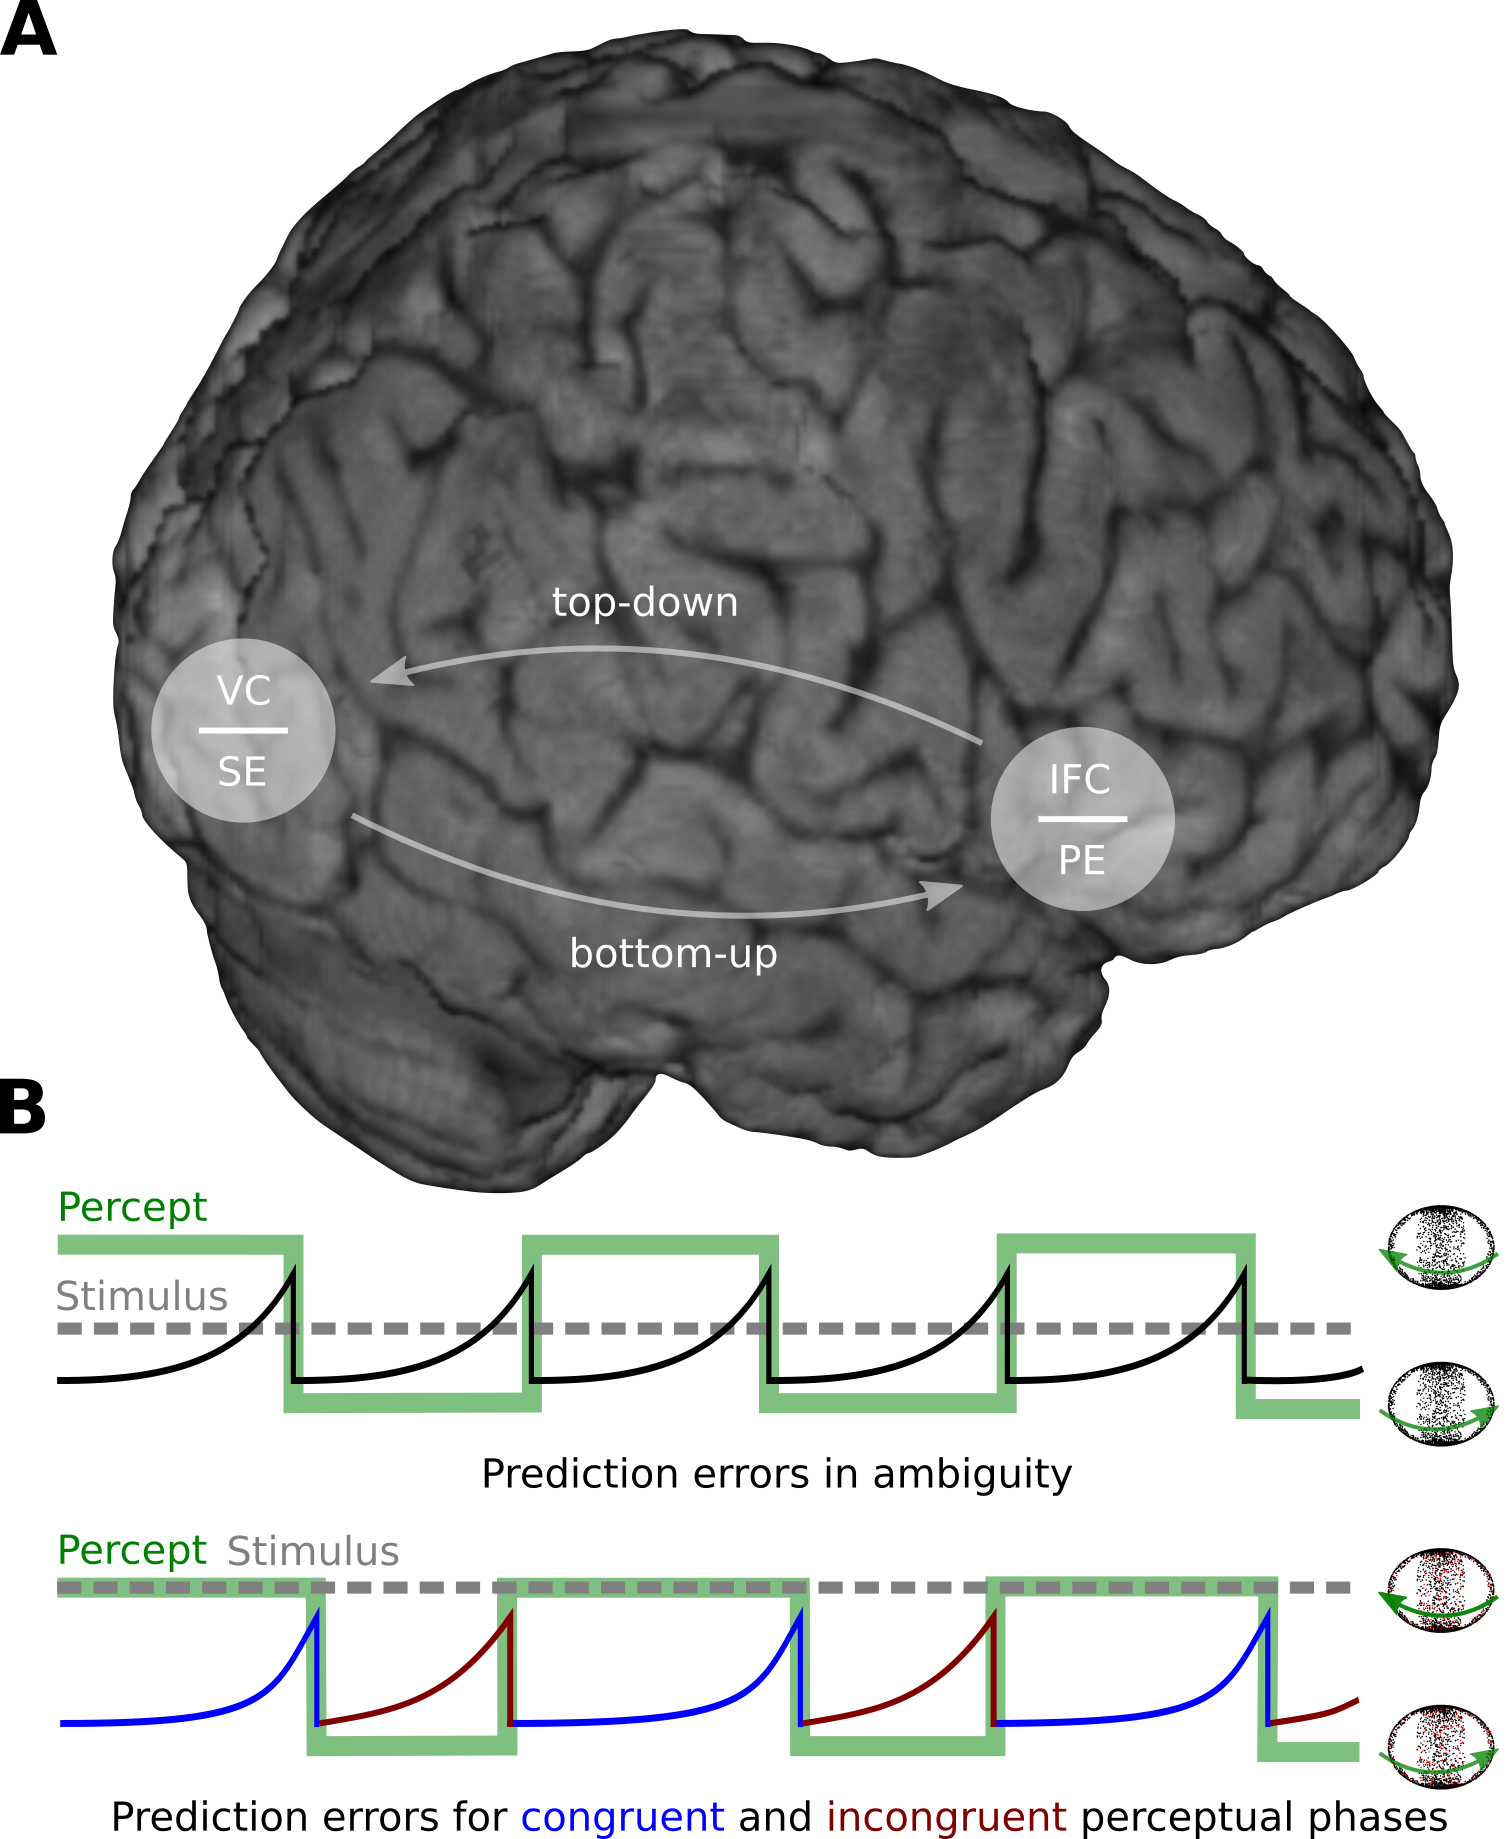
\includegraphics[width=11cm]{Figure_1.png}
\end{center}
\end{figure}

{\textbf{Figure 1. Transitions in Bistable Perception.} \textbf{A.} According to the hybrid model \parencite{Sterzer2009}, bistable perception arises from an interplay of bottom-up and top-down processes between visual cortex (VC) and inferior frontal cortex (IFC). The predictive-coding model of bistable perception \parencite{Hohwy2008a, Weilnhammer2017} mirrors this hypothesis and views transitions during bistability as a result of an integration of sensory evidence (SE) with prior beliefs about the environments’ stability, which are dynamically updated by PE signals. By parametrically modulating sensory evidence, this study seeks to test the hypothesis that IFC represents a PE signal and is hence actively implicated in perceptual transitions during bistability. \textbf{B.} Here, we depict perceptual states and associated changes in PE for bistable perception induced by a random dot structure-from-motion stimulus (RDK), whose perceived direction of rotation (green line) alternates between left- and rightward motion of the front-surface (icons on the right). In the absence of disambiguating sensory evidence (grey dotted line), the predictive coding model of bistable perception assumes escalating PEs (black solid line) during each perceptual phase and a minimization of PEs immediately after a perceptual transition. In the light of additional sensory evidence introduced by graded ambiguity (grey dotted line), perception fluctuates between perceptual phases congruent with current sensory evidence (overlap between grey dotted line and green line) and perceptual phases incongruent with current sensory evidence (divergence between grey dotted line and green line). During congruent perceptual phases, PEs are reduced (blue solid line), while incongruent perceptual phases are characterized by enhanced PEs (red solid line). Importantly, the amount of disambiguating sensory evidence determines the strength of reduction or enhancement of PEs as well as the relative duration of congruent perceptual phases.} 

\clearpage
\begin{figure}[h]
\begin{center}
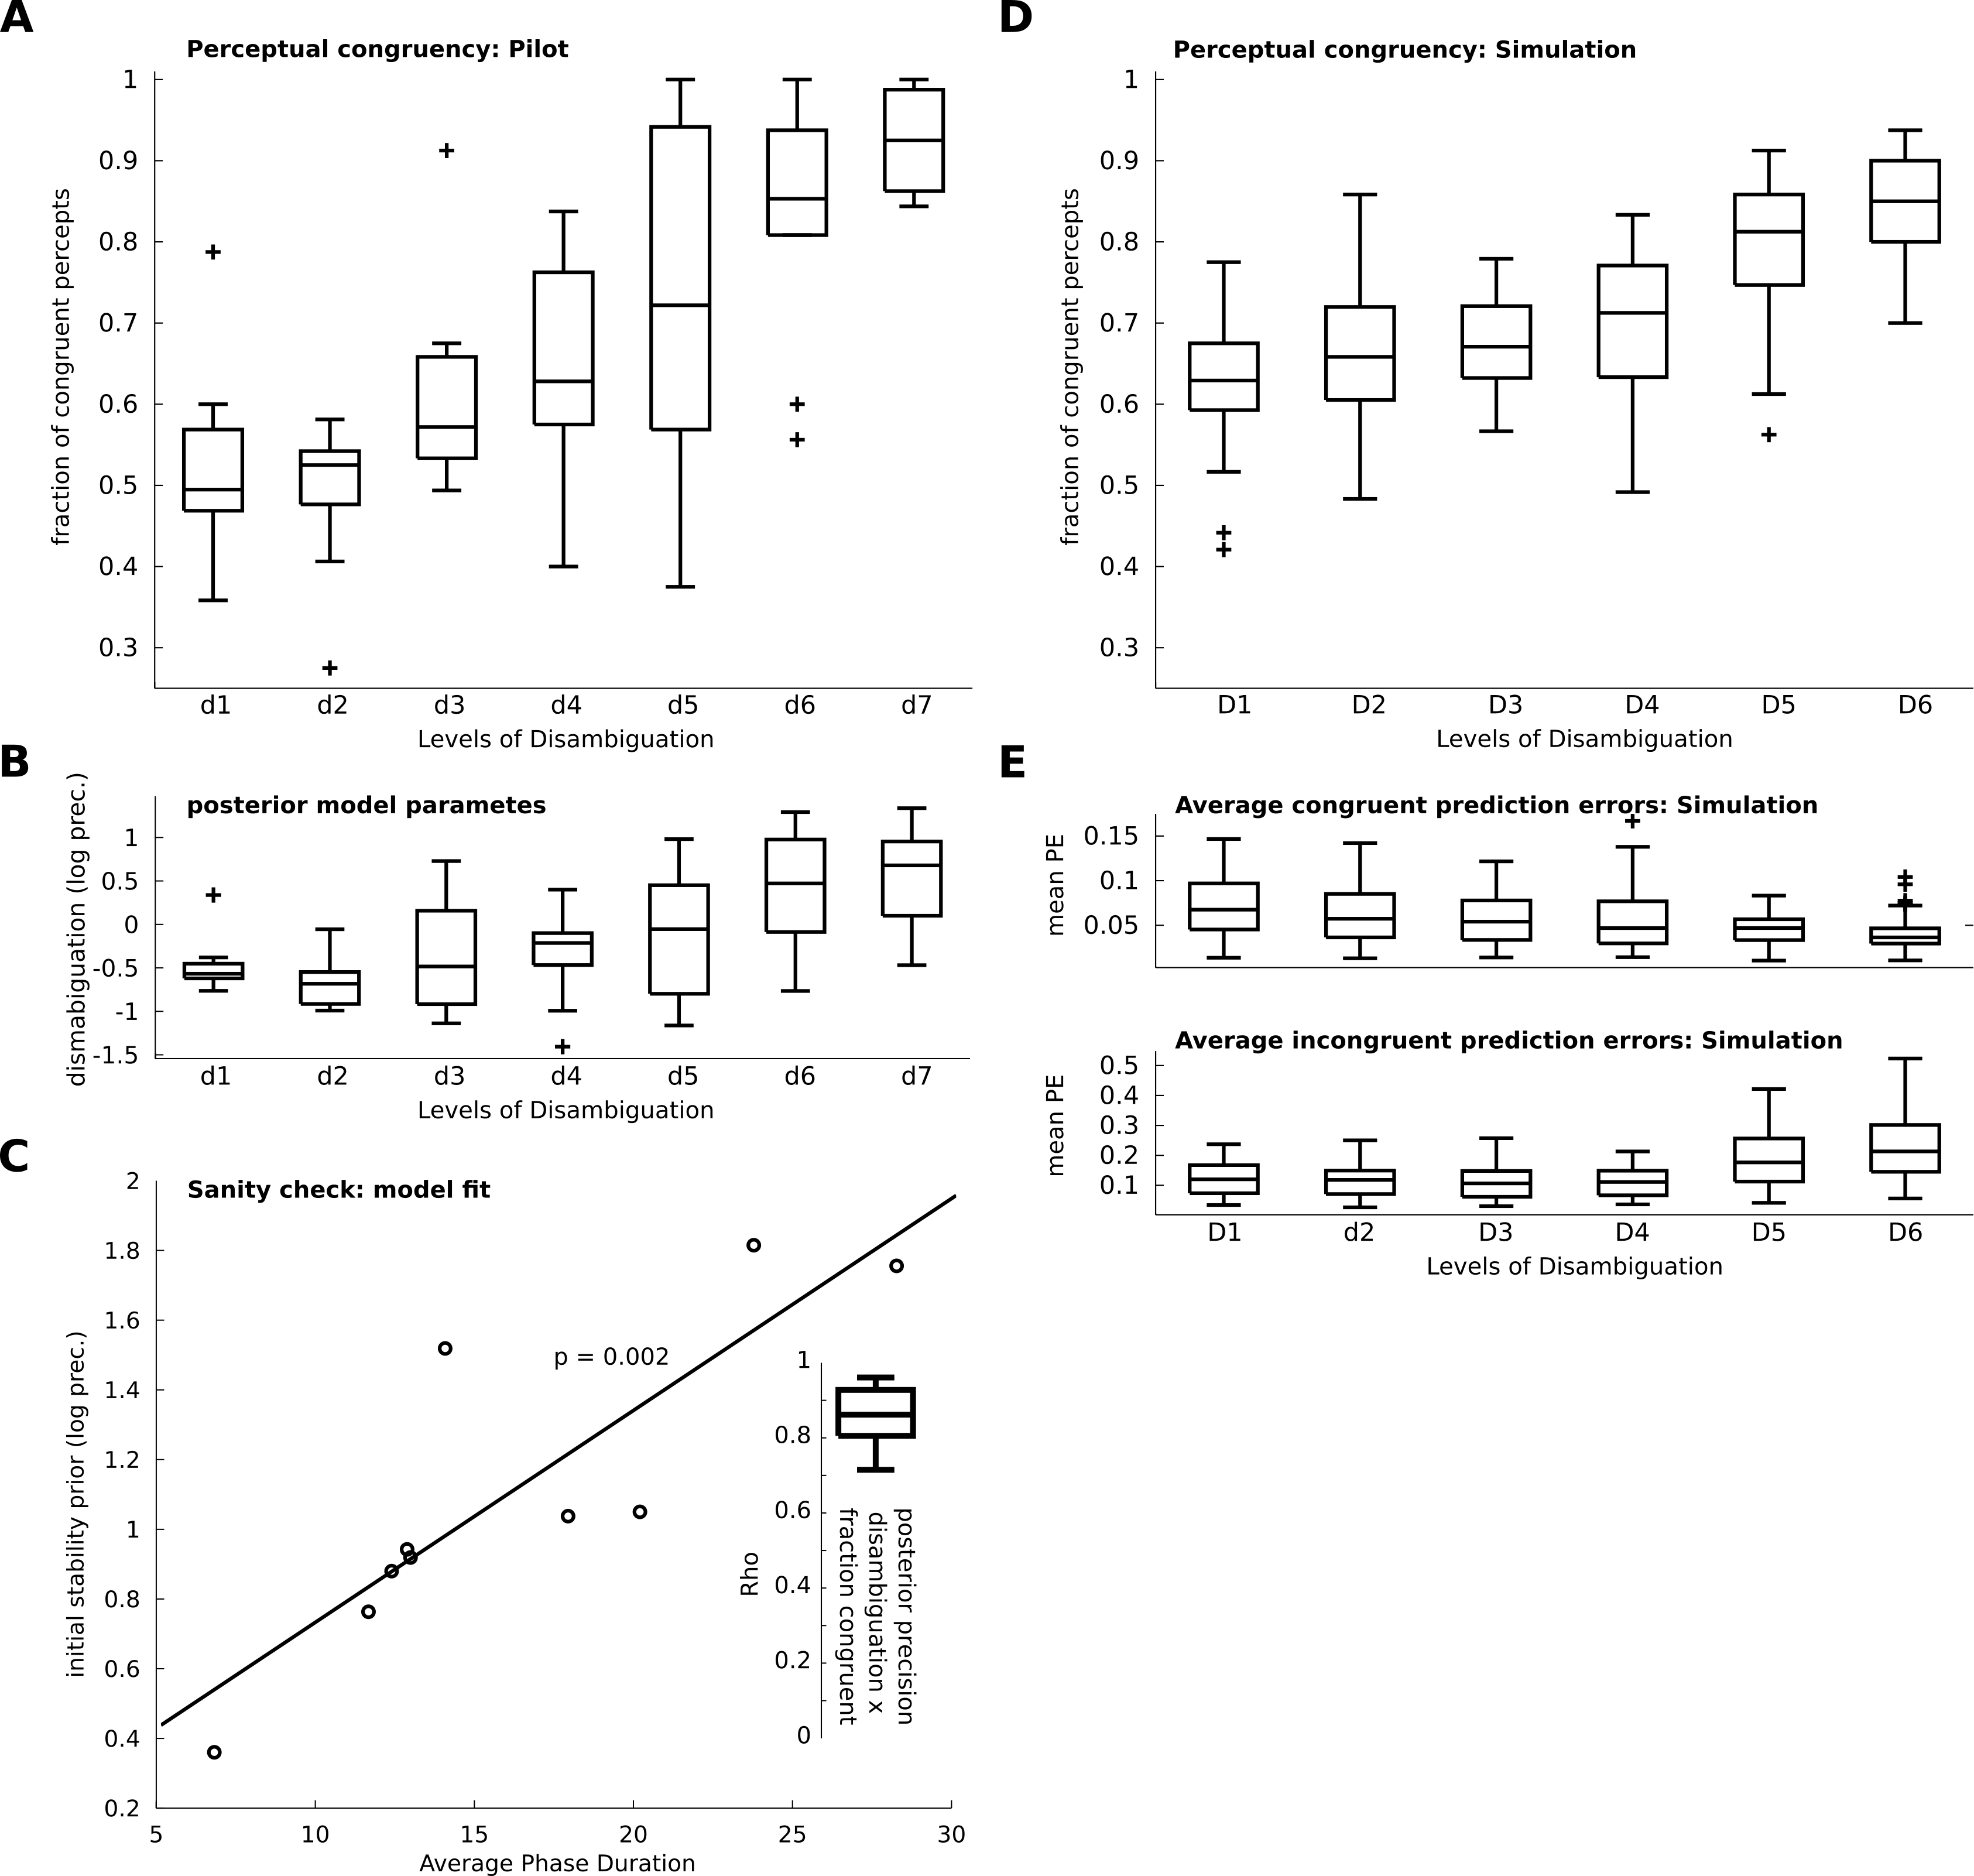
\includegraphics[width=16cm]{Figure_2.png}
\end{center}
\end{figure}

\textbf{Figure 2. Behavioural Pilot (A to C) and Simulation (D to E)}. \textbf{A.} Here, we depict the fraction of percepts congruent with current sensory evidence versus the level of disambiguation (i.e., sensory evidence, conditions d1 to d7). One-way rmANOVA indicated a significant effect of sensory evidence on perceptual congruency ($F(9) = 17.50$, $p < 1.3e-10$). \textbf{B.} By analogy, the posterior log precision of disambiguation ($\pi_{DIS d1-d7}$) increased significantly across levels of sensory evidence ($F(9) = 9.3664$, $p < 8.4405e-07$). \textbf{C}. As a sanity check for model-fit, we correlated posterior model parameters ($\pi_{IPS}$ and $\pi_{DIS d1-d7}$) with conventional measures (average phase duration and congruent percepts). As expected, average phase durations were highly correlated to $\pi_{IPS}$ ($\rho(9) = 0.85$, $p = 0.0018$, Pearson correlation). Within-participant correlation coefficients between the fraction of congruent percepts and posterior $\pi_{DIS}$ across conditions d1 to d7 were equal to 0.86 $\pm$ 0.03 (one-sample one-sided t-test against zero: $T(9) = 29.4$, $p = 1.9537e-09$). \textbf{D.} When simulating the sequence of perceptual states for six levels of disambiguation (D1 to D6), we found a significant effect of sensory evidence (i.e. conditions D1 to D6) on the fraction of congruent percepts ($F(46) = 37.635$, $p = 5.5585e-37$, one-way rmANOVA). \textbf{E}. Across levels of sensory evidence D1 to D6, average PEs are progressively reduced for congruent perceptual phases and enhanced for incongruent perceptual phases as indicated by a main effect of congruency ($F(46) = 186.540$, $p < 0.0001$) as well as by a "congruency x sensory evidence" interaction ($F(46) = 55.380$, $p < 0.0001$, two-way rmANOVAs).

\clearpage
\begin{figure}[h]
\begin{center}
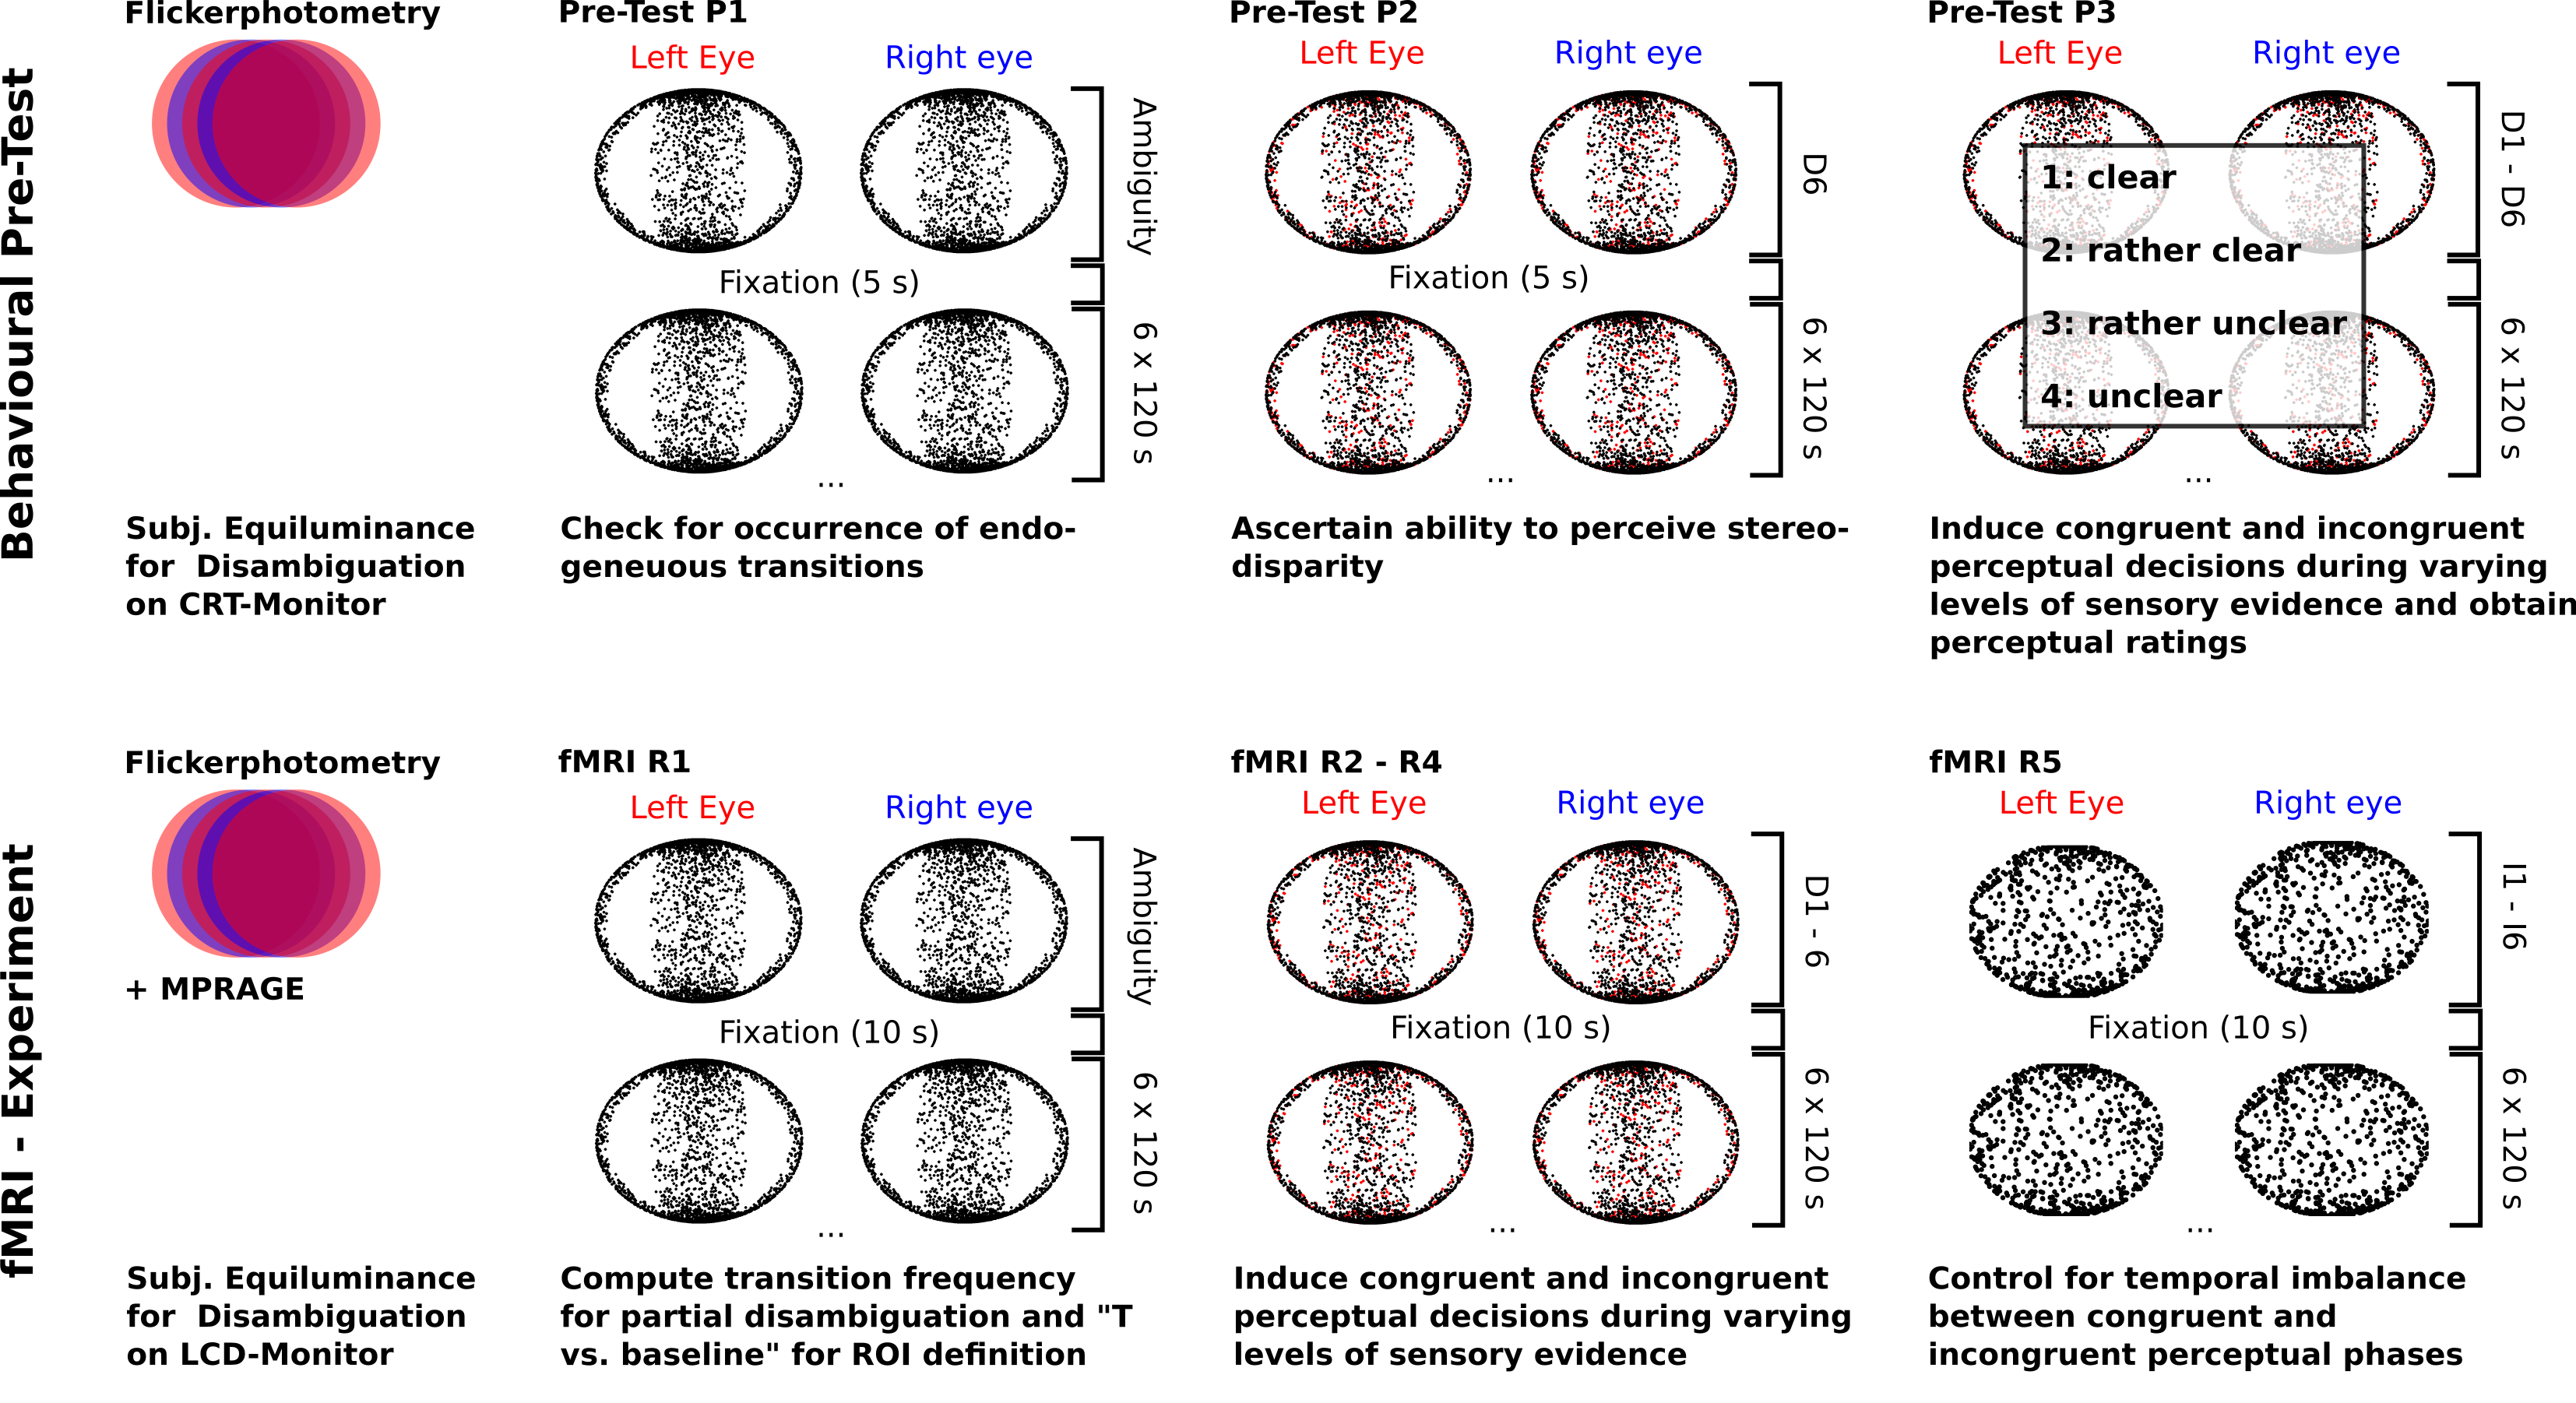
\includegraphics[width=16cm]{Figure_3.png}
\end{center}
\end{figure}

\textbf{Figure 3. Experimental Paradigm}.  The behavioural pretest consists in one run of six blocks with 120 sec of ambiguous stimulation (i.e., identical stimulation to both eyes, P1), one run of six blocks (120 sec) of fully disambiguated stimulation (P2) and one run of six blocks with 120 sec of parametrically disambiguated stimulation (P3). In the main experiment, run R1 consists in six blocks (120 sec) of fully ambiguous stimulation. The individual frequency of perceptual transitions determines the frequency of changes in the direction of parametric disambiguation in the upcoming runs R2 to R4. Here, a fraction of the dots composing the RDK (highlighted in red) is shifted between the two monocular channels, which are separated by red-blue filter-glasses. The conditions D1 to D6 are characterized by the percentage of disambiguated dots (§15\%, 30\%, 45\%, 60\%, 75\% and 100\%§) and occur in random order. Run R5 contains a control experiment assessing the effects of temporal imbalance introduced by the conditions D1 to D6 in individual participants. Here, we present leftward and rightward planar dot motion in six conditions of increasing temporal imbalance (I1 to I6), which appear in random order. All experiments are preceeded by heterochromatic flicker photometry. 


\clearpage
\begin{figure}[h]
\begin{center}
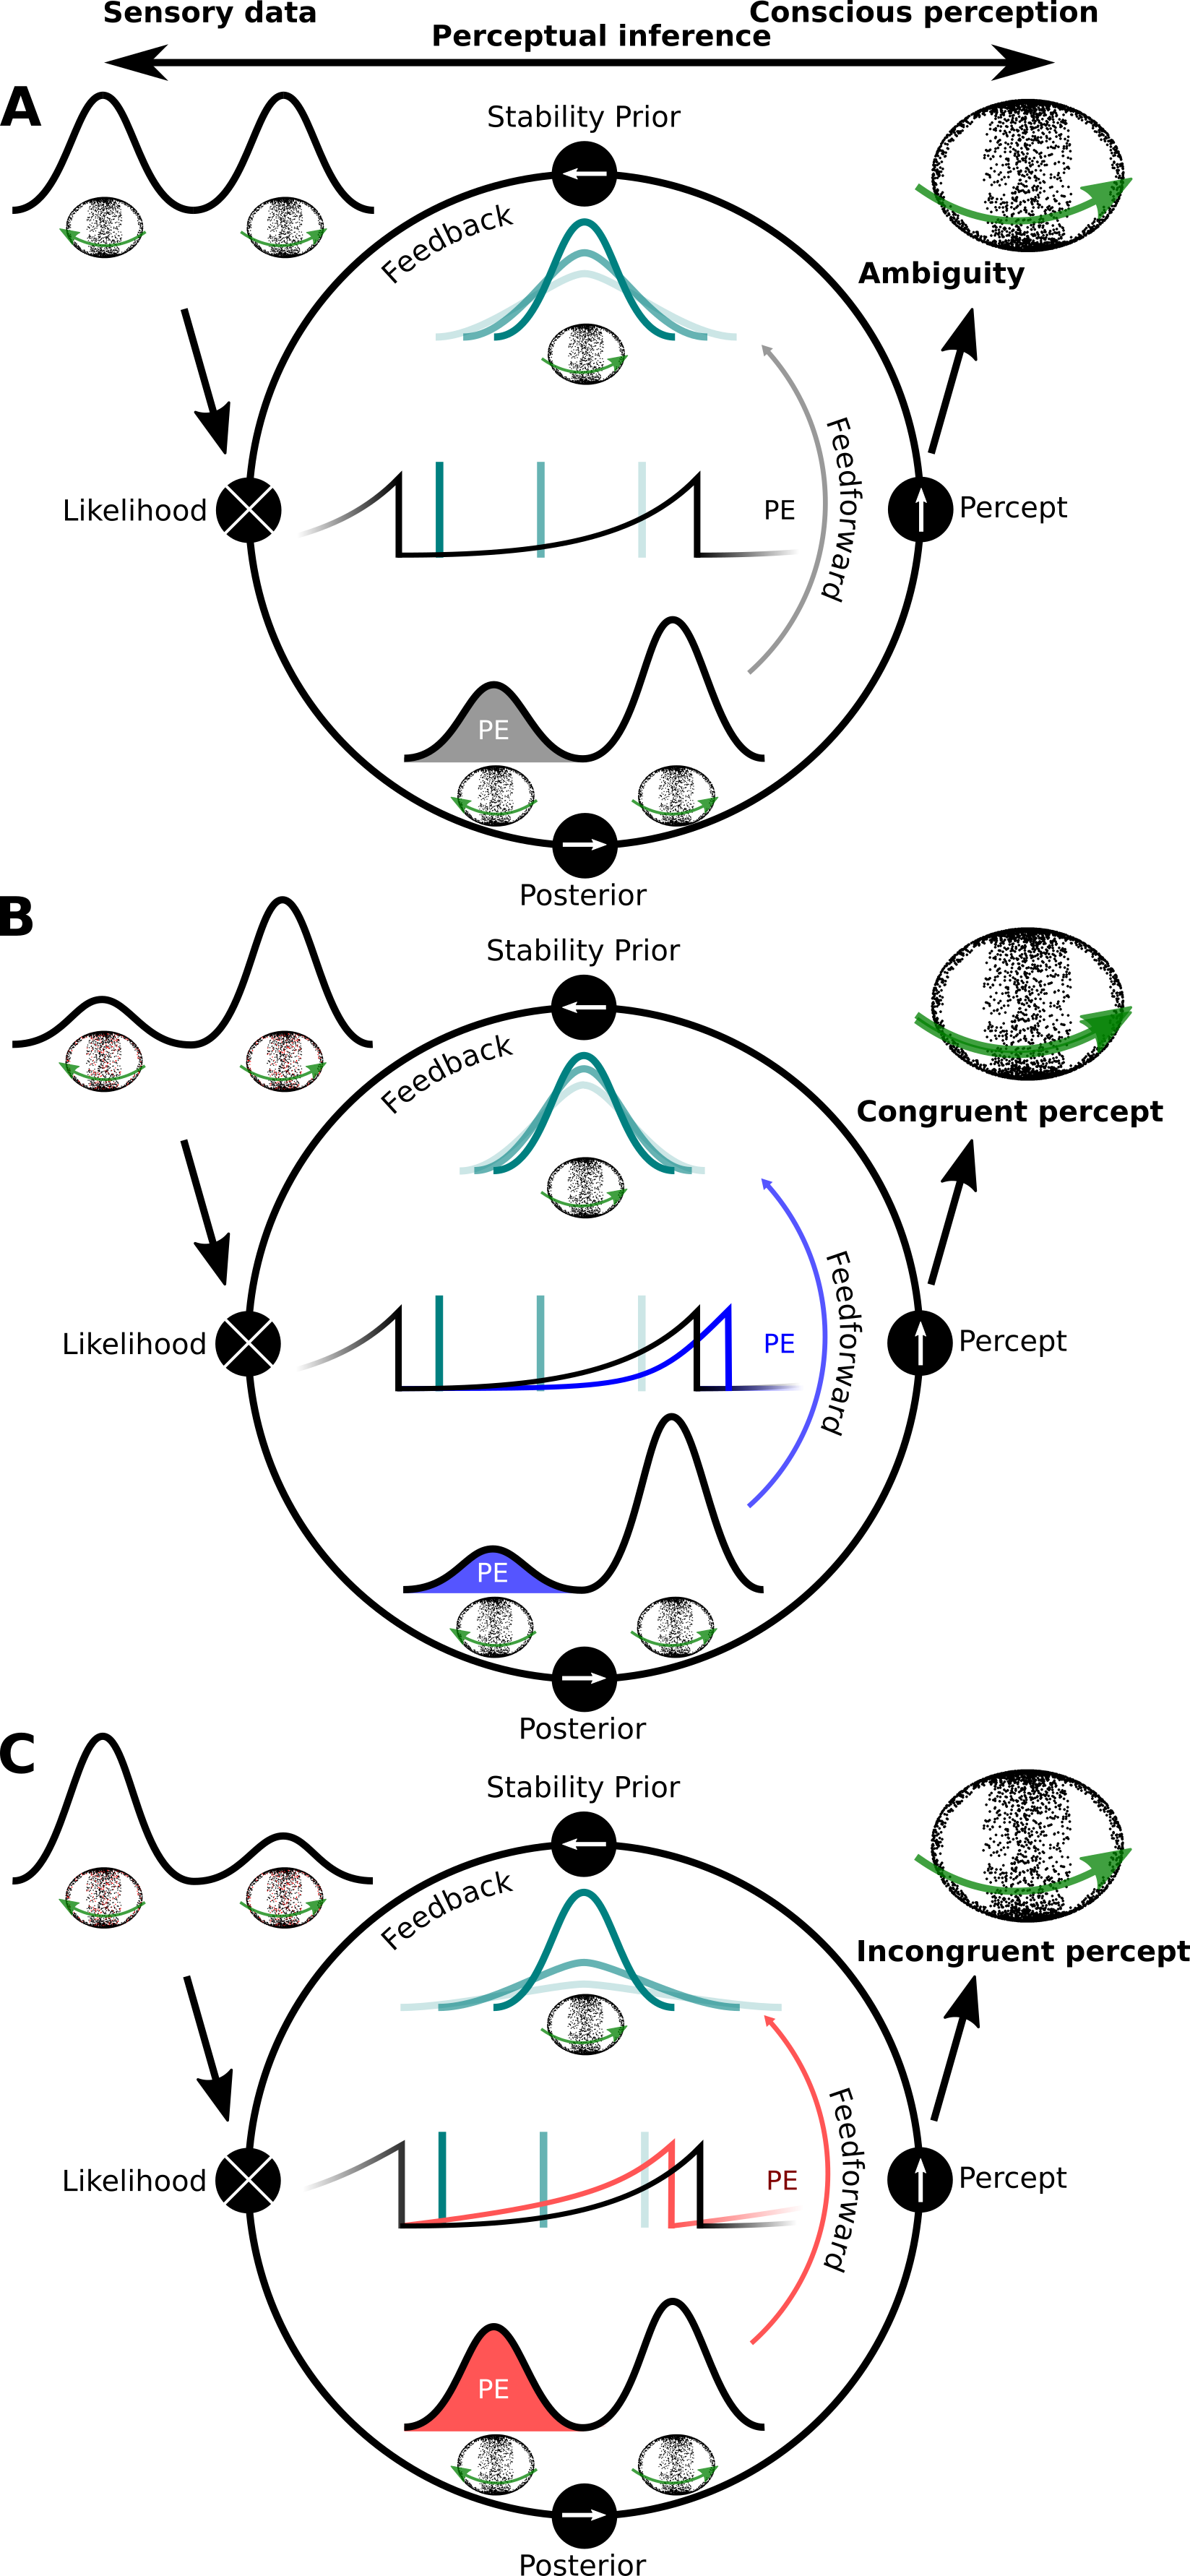
\includegraphics[width=7cm]{Figure_4.png}
\end{center}
\end{figure}

\textbf{Figure 4. Bayesian Preditive Coding Model of Bistable Perception.} This schematic depiction of the Bayesian predictive coding model of bistable perception \parencite{Weilnhammer2017} illustrates our hypothesis about the generation of conscious perception in the light of ambiguous and partially disambiguated sensory data through the process of perceptual inference. Moreover, it depicts the evolution of the prior belief in stability of the sensory environment and associated PE signals for three different situations: ambiguous stimulation (\textbf{A.}) as well as partial disambiguation congruent (\textbf{B.}) and incongruent (\textbf{C.}) with the current perceptual interpretation of the stimulus. We highlight three consecutive time-points for PEs and prior distributions in shades of blue. \textbf{A.} In this example, the participant adopts the perceptual interpretation "rotation of front-surface to the right" (right top corner). This establishes a prior belief about the stability of the perceptual environment (centre top), whose mean is centred on the current perceptual interpretation. The unimodal prior distribution is combined with the fully ambiguous sensory data (top left corner) represented by a bimodal likelihood. This results in a bimodal posterior distribution (centre bottom) representing posterior evidence for both perceptual interpretations. This distribution predicts the upcoming percept of the participant. If the participants again perceives the stimulus as rotating to the right, the residual evidence for the alternative perceptual interpretation (highlighted in grey) constitutes a PE that weakens the precision of the prior. Over time, the precision of the prior decreases, while PEs escalate, until the participant perceives a perceptual transition. At this point, the prior precision will be re-set to its initial value ($\pi_{IPS}$), which leads to a minimization of PE by virtue of the perceptual transition. \textbf{B.} Here, we describe the dynamics of our model for partially disambiguated sensory data (top left corner) that are congruent with the current perceptual interpretation. In this case, the disambiguating sensory evidence reduces the residual evidence for the alternative interpretation and the associated PE (highlighted in blue). The precision of the stability prior decreases more slowly, leading to an attenuation of PEs and a prolongation of the perceptual phase. Importantly, these effects scale with the strength of partial disambiguation of the sensory data ($\pi_{DIS}$). \textbf{C.} The antithetical example depicts the influence of partially disambiguated sensory data incongruent with the current sensory evidence. Here, disambiguating sensory evidence enhances the residual evidence for the alternative interpretation and the associated PE (highlighted in red). The precision of the stability prior decreases more rapidly, leading to a enhanced accumulation of PEs and a shortening of the perceptual phase. Again, these effects scale with the strength of partial disambiguation of the sensory data ($\pi_{DIS}$).

%%%%%%%%%%%%%%%%%%%%%%%%%%%%%%%%%%%%%%%%%%%%%%%%%%%%%%%%%%%%%%%%
%BIBLIOGRAPHY
\clearpage
\nolinenumbers

\printbibliography


  \end{document}
